% extra contents of chap4

\section{电磁延伸}

\subsection{点电荷电势推导}

\begin{gather*}
    U=\int_r^\infty k\frac{Qq}{x^2}dx=k\frac{Qq}{r}\\
    V=\frac{U}{q}=k\frac{Q}{r}
\end{gather*}

\subsection{电容器储能公式推导}

\begin{equation*}
    U=\int_0^Q\frac{q}{C}dq=\frac{Q^2}{2C}
\end{equation*}

\subsection{电容器储能损耗推导}

假设电路中除电容器以外的外阻为$R$,则回路方程为
\begin{equation*}
    E=RI+\frac{Q}{C}\implies
    \frac{dQ}{dt}=I=\frac{E-\frac{Q}{C}}{R}
\end{equation*}
对等式两边积分可得电荷量随时间变化的函数
\begin{gather*}
    \int\frac{dQ}{E-\frac{Q}{C}}=\int\frac{dt}{R}\\
    -C\log\left\lvert E-\frac{Q}{C}\right\rvert=\frac{t}{R}+\gamma\\
    E-\frac{Q}{C}=\Gamma\exp\left(\frac{t}{RC}\right)\quad\left(\Gamma=\exp\left(-\frac{\gamma}{C}\right)\right)\\
\end{gather*}
根据初始条件$(t,Q)=(0,0)$可得$\Gamma=E$,因此
\begin{equation*}
    Q(t)=CE\left(1-\exp\left(-\frac{t}{RC}\right)\right)
\end{equation*}
最后使用$W=I^2Rt$积分求解即可
\begin{gather*}
    I=\frac{dQ}{dt}=\frac{E}{R}\exp\left(-\frac{t}{RC}\right)\\
    W=\int_0^\infty I^2Rdt=\frac12CE^2
\end{gather*}

\subsection{直线电流磁场推导}

根据Biot-Savart定律可得
\begin{align*}
    \mathbf{B}=&\frac{\mu_0}{4\pi}\int_{-\infty}^{\infty}\mathbf{J}\times\frac{\mathbf{r}-\mathbf{l}}{|\mathbf{r}-\mathbf{l}|^3}d^3l\\
    =&\frac{\mu_0I}{4\pi}\int_{-\infty}^{\infty}d\mathbf{l}\times\frac{\mathbf{r}-\mathbf{l}}{|\mathbf{r}-\mathbf{l}|^3}
\end{align*}
设$(0,0,r_z)$为矢量基准点,则可简记$r=(r_x,r_y,0)$
\begin{align*}
    \mathbf{B}=&\frac{\mu_0I}{4\pi}\int_{-\infty}^{\infty}dl\cdot e_z\times\frac{r_xe_x+r_ye_y-le_z}{|r^2+l^2|^{3/2}}\\
    =&\frac{\mu_0I}{4\pi}\int_{-\infty}^{\infty}dl\frac{r_xe_y-r_ye_x}{|r^2+l^2|^{3/2}}
\end{align*}
关于$l$求解反常积分可得
\begin{align*}
    \mathbf{B}=&\frac{\mu_0I}{4\pi}\left[\frac{l(r_xe_y-r_ye_x)}{r^2\sqrt{r^2+l^2}}\right]_{-\infty}^{\infty}\\
    =&\frac{\mu_0I}{2\pi r^2}(r_xe_y-r_ye_x)
\end{align*}
将结果改写为位置向量的形式
\begin{equation*}
    \mathbf{B}=\frac{\mu_0I}{2\pi r^2}(-r_y,r_x,0)
\end{equation*}
即大小为$B=\frac{\mu_0I}{2\pi r}$,方向与$\mathbf{r}$垂直的磁场。

另外,倘若使用Ampère's circuital law则可以更加方便地求解。
\begin{align*}
    \oint_{\partial S}B\cdot dl=&\mu_0I\\
    2\pi r B=&\mu_0I\\
    B=&\frac{\mu_0I}{2\pi r}
\end{align*}

\subsection{环形电流磁场推导}

设位于xy平面上的环形电流半径为$r$,计算z轴上点$\mathbf{z}=(0,0,z)$处的磁场。则根据Biot-Savart定律$\mathbf{l}=(l\cos\phi,l\sin\phi,0)$处的微小电流产生的磁场即为
\begin{align*}
    d\mathbf{B}=&\frac{\mu_0I}{4\pi}\frac{d\mathbf{l}\times(\mathbf{z}-\mathbf{l})}{|\mathbf{z}-\mathbf{l}|^3}\\
    =&\frac{\mu_0I}{4\pi|\mathbf{z}-\mathbf{l}|^3}(-\sin\phi,\cos\phi,0)dl\times(-l\cos\phi,-l\sin\phi,r)\\
    =&\frac{\mu_0I}{4\pi|\mathbf{z}-\mathbf{l}|^3}(r\cos\phi,r\sin\phi,l)dl
\end{align*}
分别关于xyz三个方向积分可得
\begin{align*}
    \begin{cases}
        B_x=\frac{\mu_0}{4\pi}\oint\frac{z\cos\phi}{|\mathbf{z}-\mathbf{l}|^3}dl
        =\frac{\mu_0}{4\pi}\int_0^{2\pi}\frac{z\cos\phi}{|\mathbf{z}-\mathbf{l}|^3}ld\phi=0\\
        B_y=\frac{\mu_0}{4\pi}\oint\frac{z\sin\phi}{|\mathbf{z}-\mathbf{l}|^3}dl=0\\
        B_z=\frac{\mu_0}{4\pi}\oint\frac{l}{|\mathbf{z}-\mathbf{l}|^3}dl
        =\frac{\mu_0}{4\pi}\oint\frac{ldl}{(z^2+l^2)^{3/2}}=\frac{\mu_0Il^2}{2(z^2+l^2)^{3/2}}\\
    \end{cases}
\end{align*}
可见除$B_z$以外的磁场均为0,并且当$z=0$时$B_z=\frac{\mu_0I}{2l}$的确成立。

\subsection{线圈磁场推导}

\begin{figure}[ht!]
    \centering
    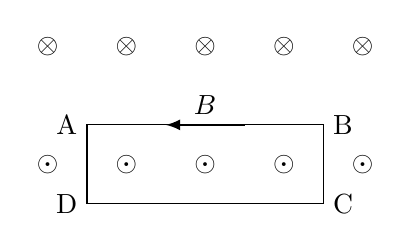
\begin{tikzpicture}
        \foreach \x in {0,...,4} {
            \node at (\x, 0) {$\odot$};
            \node at (\x, 1.5) {$\otimes$};
        }
        \draw (0.5,-0.5) -- (0.5,0.5) node[left] {A} -- (3.5,0.5) node[right] {B} -- (3.5,-0.5) node[right] {C} -- (0.5,-0.5) node[left] {D} --cycle;
        \draw[thick, -latex] (2.5,0.5) -- node[above] {$B$} (1.5,0.5);
    \end{tikzpicture}
    \caption{线圈磁场截面}
\end{figure}
如图所示,确定一个固定路径,采用Ampère's circuital law进行计算。
\begin{gather*}
    \oint_{\partial S}B\cdot dl=\mu_0\int_Sj\cdot dS\\
    \underline{Bl}_{AB}+\underline{0}_{BC}+\underline{0}_{CD}+\underline{0}_{DA}=\mu_0I\cdot nl\\
    B=\mu_0nI
\end{gather*}

\subsection{洛伦兹力推导}

使用电流的微观定义计算单个载流子的受力即可。
\begin{align*}
    \vec{f}=&\frac{\vec{F}}{N}=\frac{I\vec{l}\times\vec{B}}{N}\\
    =&\frac{nqSl\vec{v}\times\vec{B}}{nSl}\\
    =&q\vec{v}\times\vec{B}
\end{align*}

\subsection{带电粒子在磁场中运动轨迹推导}

在静磁场中带电粒子的运动方程为
\begin{equation*}
    m\frac{d^2\mathbf{r}}{dt^2}=q\frac{d\mathbf{r}}{dt}\times\mathbf{B}
\end{equation*}
假设该静磁场只存在于z方向,即$\mathbf{B}=(0,0,B)$
\begin{equation*}
    m\begin{pmatrix}
     \ddot{x}\\\ddot{y}\\\ddot{z}   
    \end{pmatrix}=
    q\begin{pmatrix}
        \dot{x}\\\dot{y}\\\dot{z}
    \end{pmatrix}\times
    \begin{pmatrix}
        0\\0\\B
    \end{pmatrix}=
    qB\begin{pmatrix}
        \dot{y}\\-\dot{x}\\0
    \end{pmatrix}
\end{equation*}
其中z方向的运动方程为$m\ddot{z}=0$,即粒子在z方向做匀速直线运动。而后,使用极坐标系处理xy平面的运动,基于其转换关系
\begin{itemize}
    \item 速度:$\begin{cases}v_r=\dot{r}\\v_\phi=r\dot{\phi}\end{cases}$
    \item 加速度:$\begin{cases}a_r=\ddot{r}-r\dot{\phi}^2\\a_\phi=2\dot{r}\dot{\phi}+r\ddot{\phi}\end{cases}$
\end{itemize}
即
\begin{align*}
    \begin{cases}
        a_r=a_x\cos\phi+a_y\sin\phi
        =\frac{qB}{m}\left(v_y\cos\phi-v_x\sin\phi\right)
        =\frac{qB}{m}v_\phi\\
        a_\phi=-a_x\sin\phi+a_y\cos\phi
        =-\frac{qB}{m}\left(-v_y\sin\phi+v_x\cos\phi\right)
        =-\frac{qB}{m}v_r\\
    \end{cases}
\end{align*}
代入运动方程可得
\begin{equation*}
    \begin{cases}
        \ddot{r}-r\dot{\phi}^2=\frac{qB}{m}r\dot{\phi}\\
        2\dot{r}\dot{\phi}+r\ddot{\phi}=-\frac{qB}{m}\dot{r}
    \end{cases}
    \implies
    \begin{cases}
        \frac{\ddot{r}}{r}=\dot{\phi}\left(\frac{qB}{m}+\dot{\phi}\right)\\
        \ddot{\phi}=-\frac{\dot{r}}{r}\left(\frac{qB}{m}+2\dot{\phi}\right)
    \end{cases}
\end{equation*}
其中一式左右两边变量完全独立,因此可以拆成两个分别等于零的式子
\begin{equation*}
    \begin{cases}
        \frac{\ddot{r}}{r}=0\\
        \dot{\phi}\left(\frac{qB}{m}+\dot{\phi}\right)=0\\
        \ddot{\phi}=-\frac{\dot{r}}{r}\left(\frac{qB}{m}+2\dot{\phi}\right)
    \end{cases}
\end{equation*}
求解联立微分方程组可得
\begin{equation*}
    \begin{cases}
        \ddot{r}=0\\
        \dot{\phi}=-\frac{qB}{m}\\
        \dot{r}=0
    \end{cases}
\end{equation*}
其物理意义即为粒子在r方向上不受力、在$\phi$方向上保持恒定角速度$\frac{qB}{m}$做圆周运动。再结合z方向的匀速直线运动可知,粒子在空间上的轨迹为圆柱螺线。

\subsection{含自感直流电路的电流表达式推导}

结合自感电势和基尔霍夫定律可得
\begin{equation*}
    E-IR+V=0
\end{equation*}
即
\begin{equation*}
    \frac{dI}{dt}=\frac{E-IR}{L}
\end{equation*}
此微分方程可解
\begin{equation*}
    I=\frac{E}{R}\left(1+C\exp\left(-\frac{R}{L}t\right)\right)
\end{equation*}
在初始条件$(t,I)=(0,0)$下可知
\begin{equation*}
    I=\frac{E}{R}\left(1-\exp\left(-\frac{R}{L}t\right)\right)
\end{equation*}

\subsection{自感线圈储能公式推导}

\begin{equation*}
    U=W=qV
    =\int_0^I(Idt)\left(L\frac{dI}{dt}\right)
    =\frac12LI^2
\end{equation*}

\subsection{交流电平均电功率推导}

\begin{equation*}
    P=\frac{W}{T}
    =\frac1T\int_0^TI_0V_0\sin^2\omega tdt
    =\frac12I_0V_0
\end{equation*}

\subsection{交流电电容器结论推导}

\paragraph{电流} $I=\frac{dQ}{dt}=\frac{d(CV_0\sin\omega t)}{dt}=\omega CV_0\cos\omega t$

\paragraph{平均功率} $\bar{P}=IV=\frac1T\int_0^TI_0V_0\cos\omega t\sin\omega tdt=0$

\subsection{交流电线圈结论推导}

\paragraph{电流} 根据自感线圈电压表达式以及基尔霍夫定律可得
\begin{equation*}
    V_0\sin\omega t-L\frac{dI}{dt}=0
\end{equation*}
整理后可得
\begin{equation*}
    dI=\frac{V_0}{L}\sin\omega tdt
\end{equation*}
即
\begin{equation*}
    I=-\frac{V_0}{\omega L}\cos\omega t
\end{equation*}

\paragraph{平均功率} $\bar{P}=IV=-\frac1T\int_0^TI_0V_0\cos\omega t\sin\omega tdt=0$
